\documentclass[aspectratio=169,11pt]{beamer}

\usetheme{Madrid}
\usecolortheme{default}
\usefonttheme{professionalfonts}
\setbeamertemplate{navigation symbols}{}
\setbeamertemplate{footline}[frame number]

\usepackage{amsmath, amssymb, booktabs, graphicx}
\graphicspath{{../../assets/figures/}{assets/figures/}}

\title{Labor Regulation, Enforcement, and Insurance}
\subtitle{Labor II --- Week 9}
\author{Teaching deck draft}
\date{}

\begin{document}

\begin{frame}
  \titlepage
\end{frame}

\begin{frame}{Central question and week repositioning}
\begin{itemize}
    \item Week 9 asks how labor economists should study labor regulation as a coherent field rather than a bucket of policies.
    \item The core objects are contracting, separations, compliance, search, insurance, and information.
    \item The lecture sits between Week 8 institutions and Week 10 aggregate adjustment because regulation changes both.
\end{itemize}
\end{frame}

\begin{frame}{Week 8 to Week 9 bridge}
\begin{itemize}
    \item Week 7: wage floors as targeted wage-setting rules.
    \item Week 8: collective bargaining as organized worker voice inside the employment relationship.
    \item Week 9: the broader legal environment for dismissal, compliance, insurance, and information.
    \item Week 10 will scale these mechanisms up to layoffs, recalls, vacancies, and aggregate shocks.
\end{itemize}
\end{frame}

\begin{frame}{The four questions for the week}
\begin{enumerate}
    \item What is a useful taxonomy of labor regulations?
    \item How do policies affect workers, firms, and regulators simultaneously?
    \item When are laws effective once enforcement, salience, and uncovered margins matter?
    \item What are the spillover, inequality, and welfare implications?
\end{enumerate}
\end{frame}

\begin{frame}{General taxonomy of labor regulations}
\begin{center}
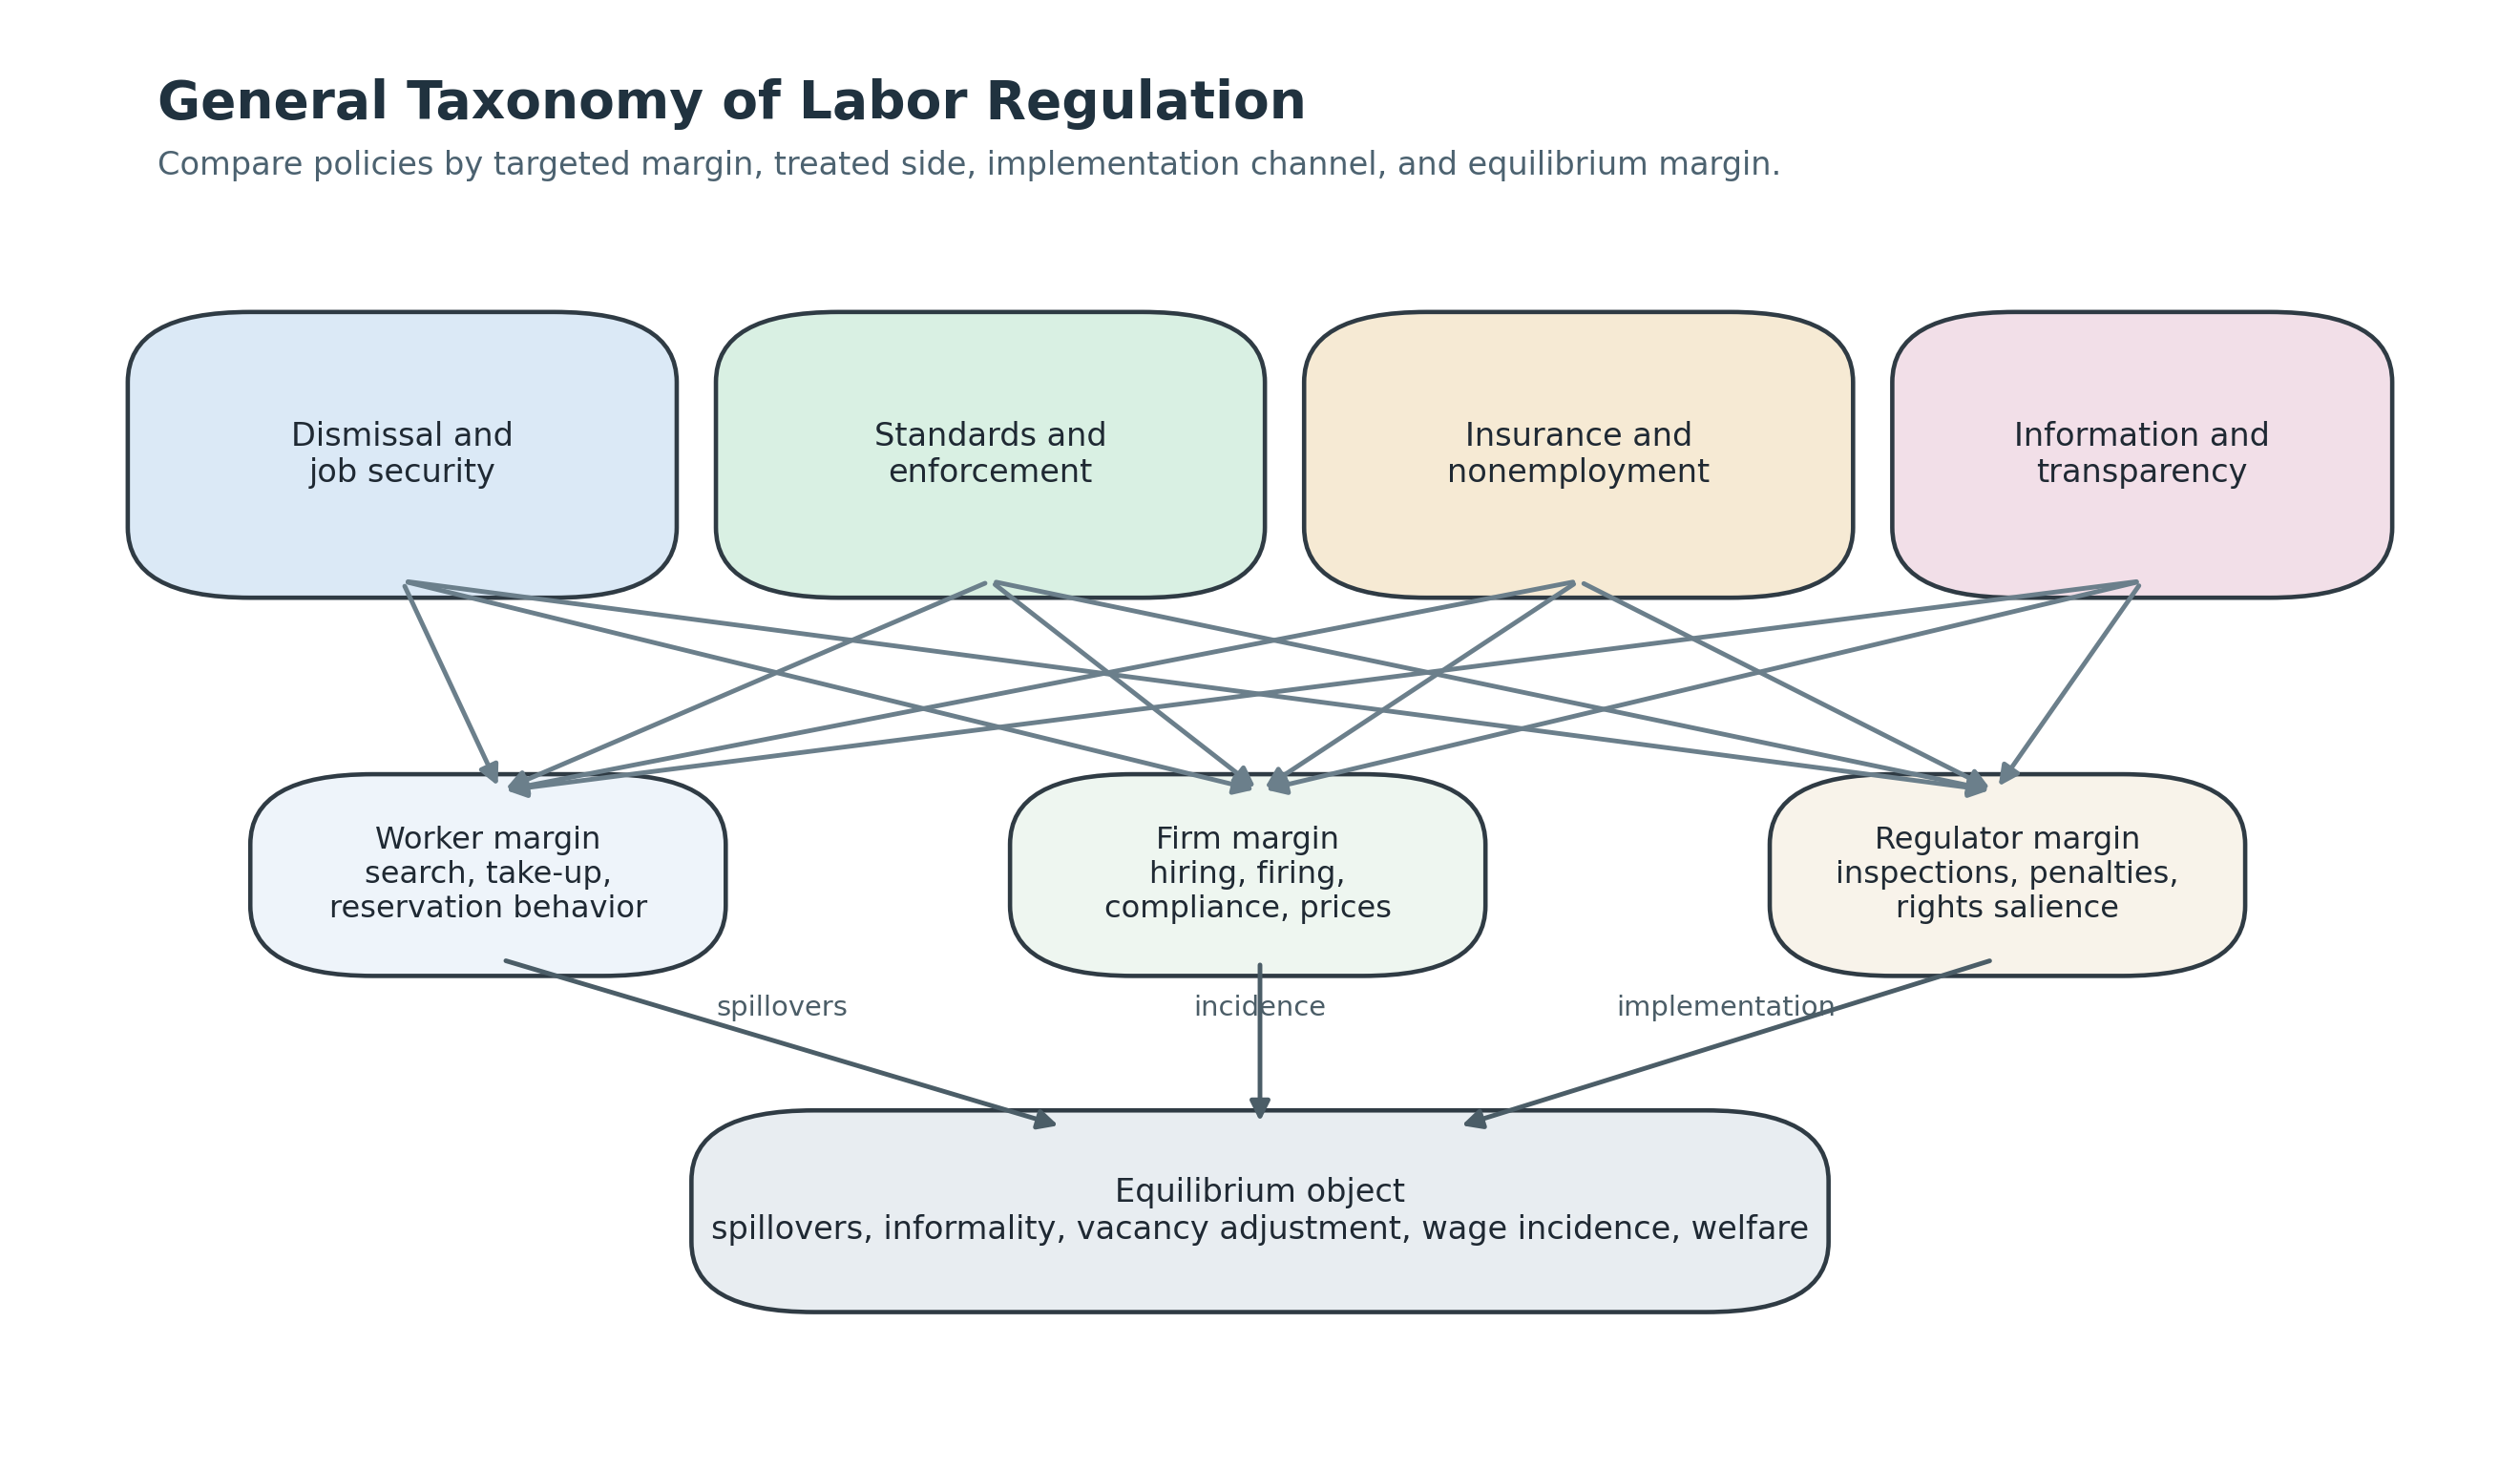
\includegraphics[height=0.74\textheight]{09-regulation-taxonomy-framework.png}
\end{center}
\end{frame}

\begin{frame}{A common regulation wedge}
\[
w_{it}^{net} = w_{it}^{gross} + b_{it} - \tau_{it}^{worker},
\qquad
c_{it}^{firm} = w_{it}^{gross} + \tau_{it}^{firm} + \kappa_{it}^{comp}
\]

\begin{itemize}
    \item Regulations change the mapping between worker value, firm labor cost, and transfers.
    \item Some policies move benefits, some penalties, some compliance costs, and some beliefs.
    \item The first question is which wedge moves and which margin absorbs it.
\end{itemize}
\end{frame}

\begin{frame}{Worker-side, firm-side, and regulator-side margins}
\begin{center}
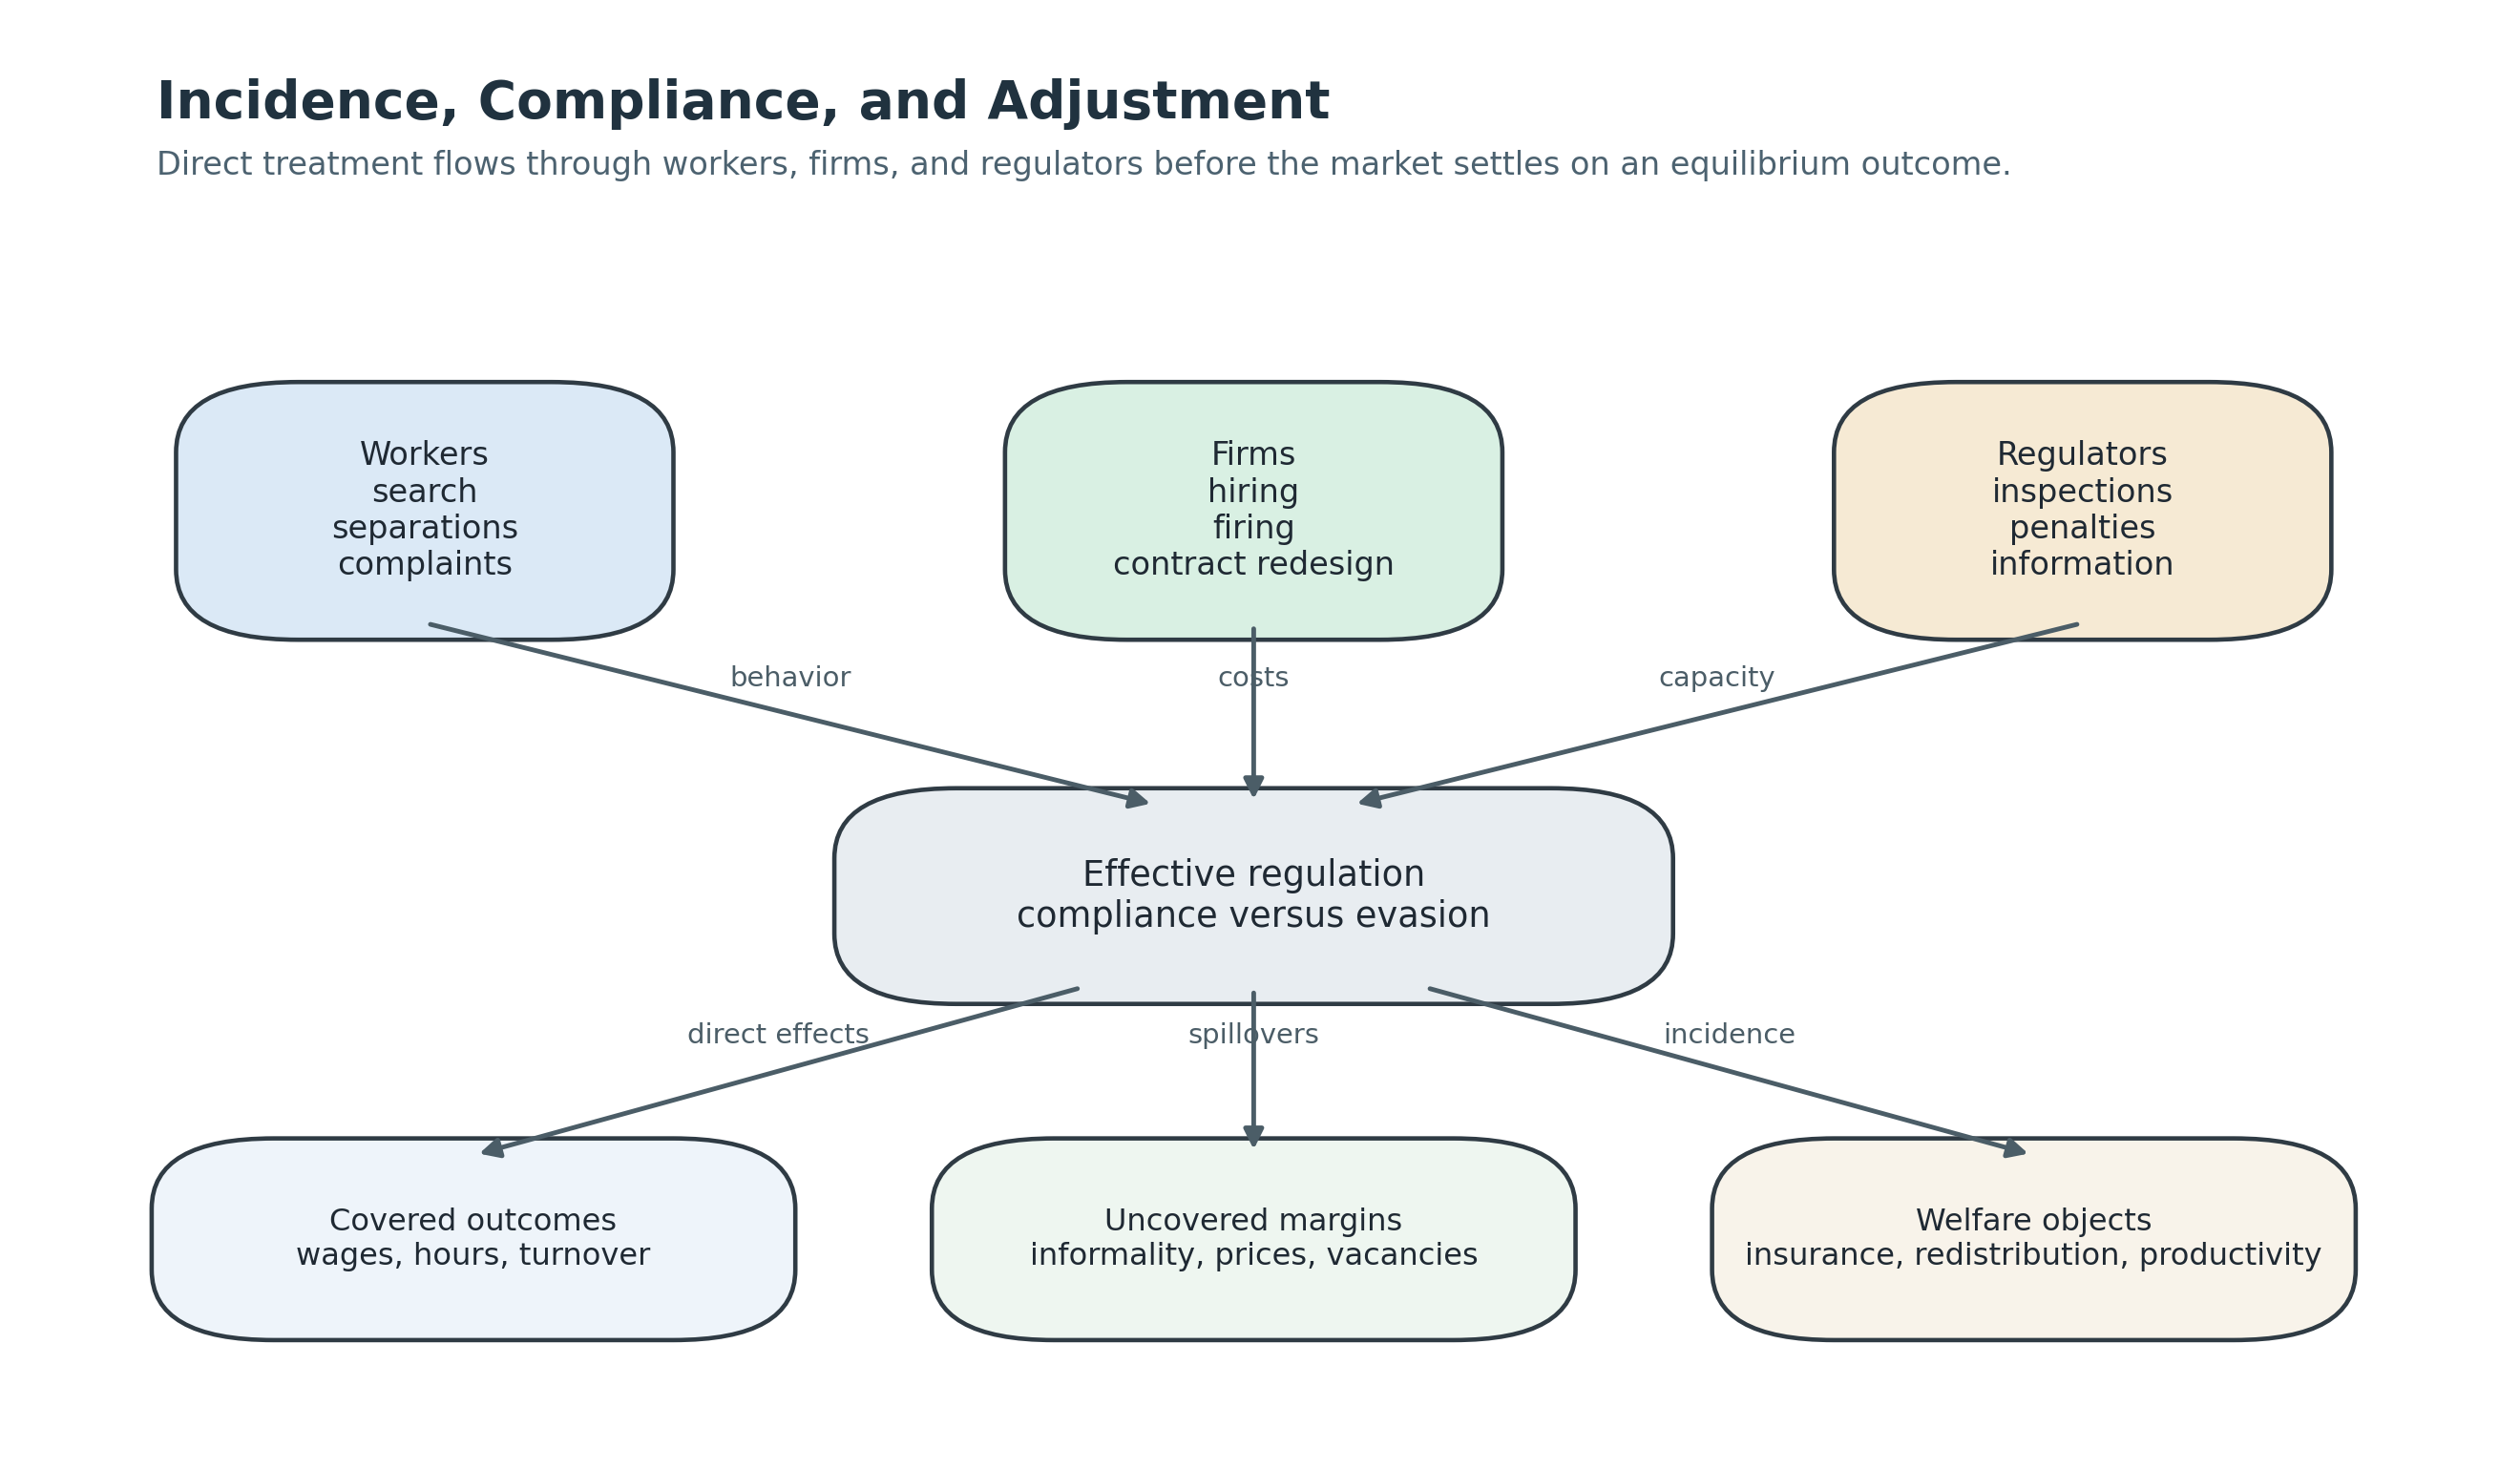
\includegraphics[height=0.68\textheight]{09-incidence-compliance-and-adjustment.png}
\end{center}
\begin{itemize}
    \item Direct treatment is not the whole policy object.
    \item Vacancies, prices, informal work, and contract substitution are equilibrium margins.
\end{itemize}
\end{frame}

\begin{frame}{Employment protection and dismissal costs}
\[
J_{jt}(s) = p_{jt} - c_{jt}^{firm} - \phi^{D}_{jt}\mathbf{1}\{s=1\}
\]

\begin{itemize}
    \item Higher dismissal costs can reduce job destruction and reduce job creation.
    \item Relevant observed margins: job flows, tenure, temporary contracts, entry, and productivity.
    \item Autor-Donohue-Schwab and Autor-Kerr-Kugler use state legal variation to study these wedges.
\end{itemize}
\end{frame}

\begin{frame}{Law on the books versus effective regulation}
\[
R_{rt}^{eff} = R_{rt}^{law} \times E_{rt} \times K_{rt} \times P_{rt}
\]

\begin{itemize}
    \item Effective regulation depends on enforcement, knowledge, and compliance.
    \item The same legal rule can bind strongly in one place and weakly in another.
    \item This is why inspections, complaints, and salience are first-order labor-market objects.
\end{itemize}
\end{frame}

\begin{frame}{Enforcement, compliance, and capacity}
\begin{center}
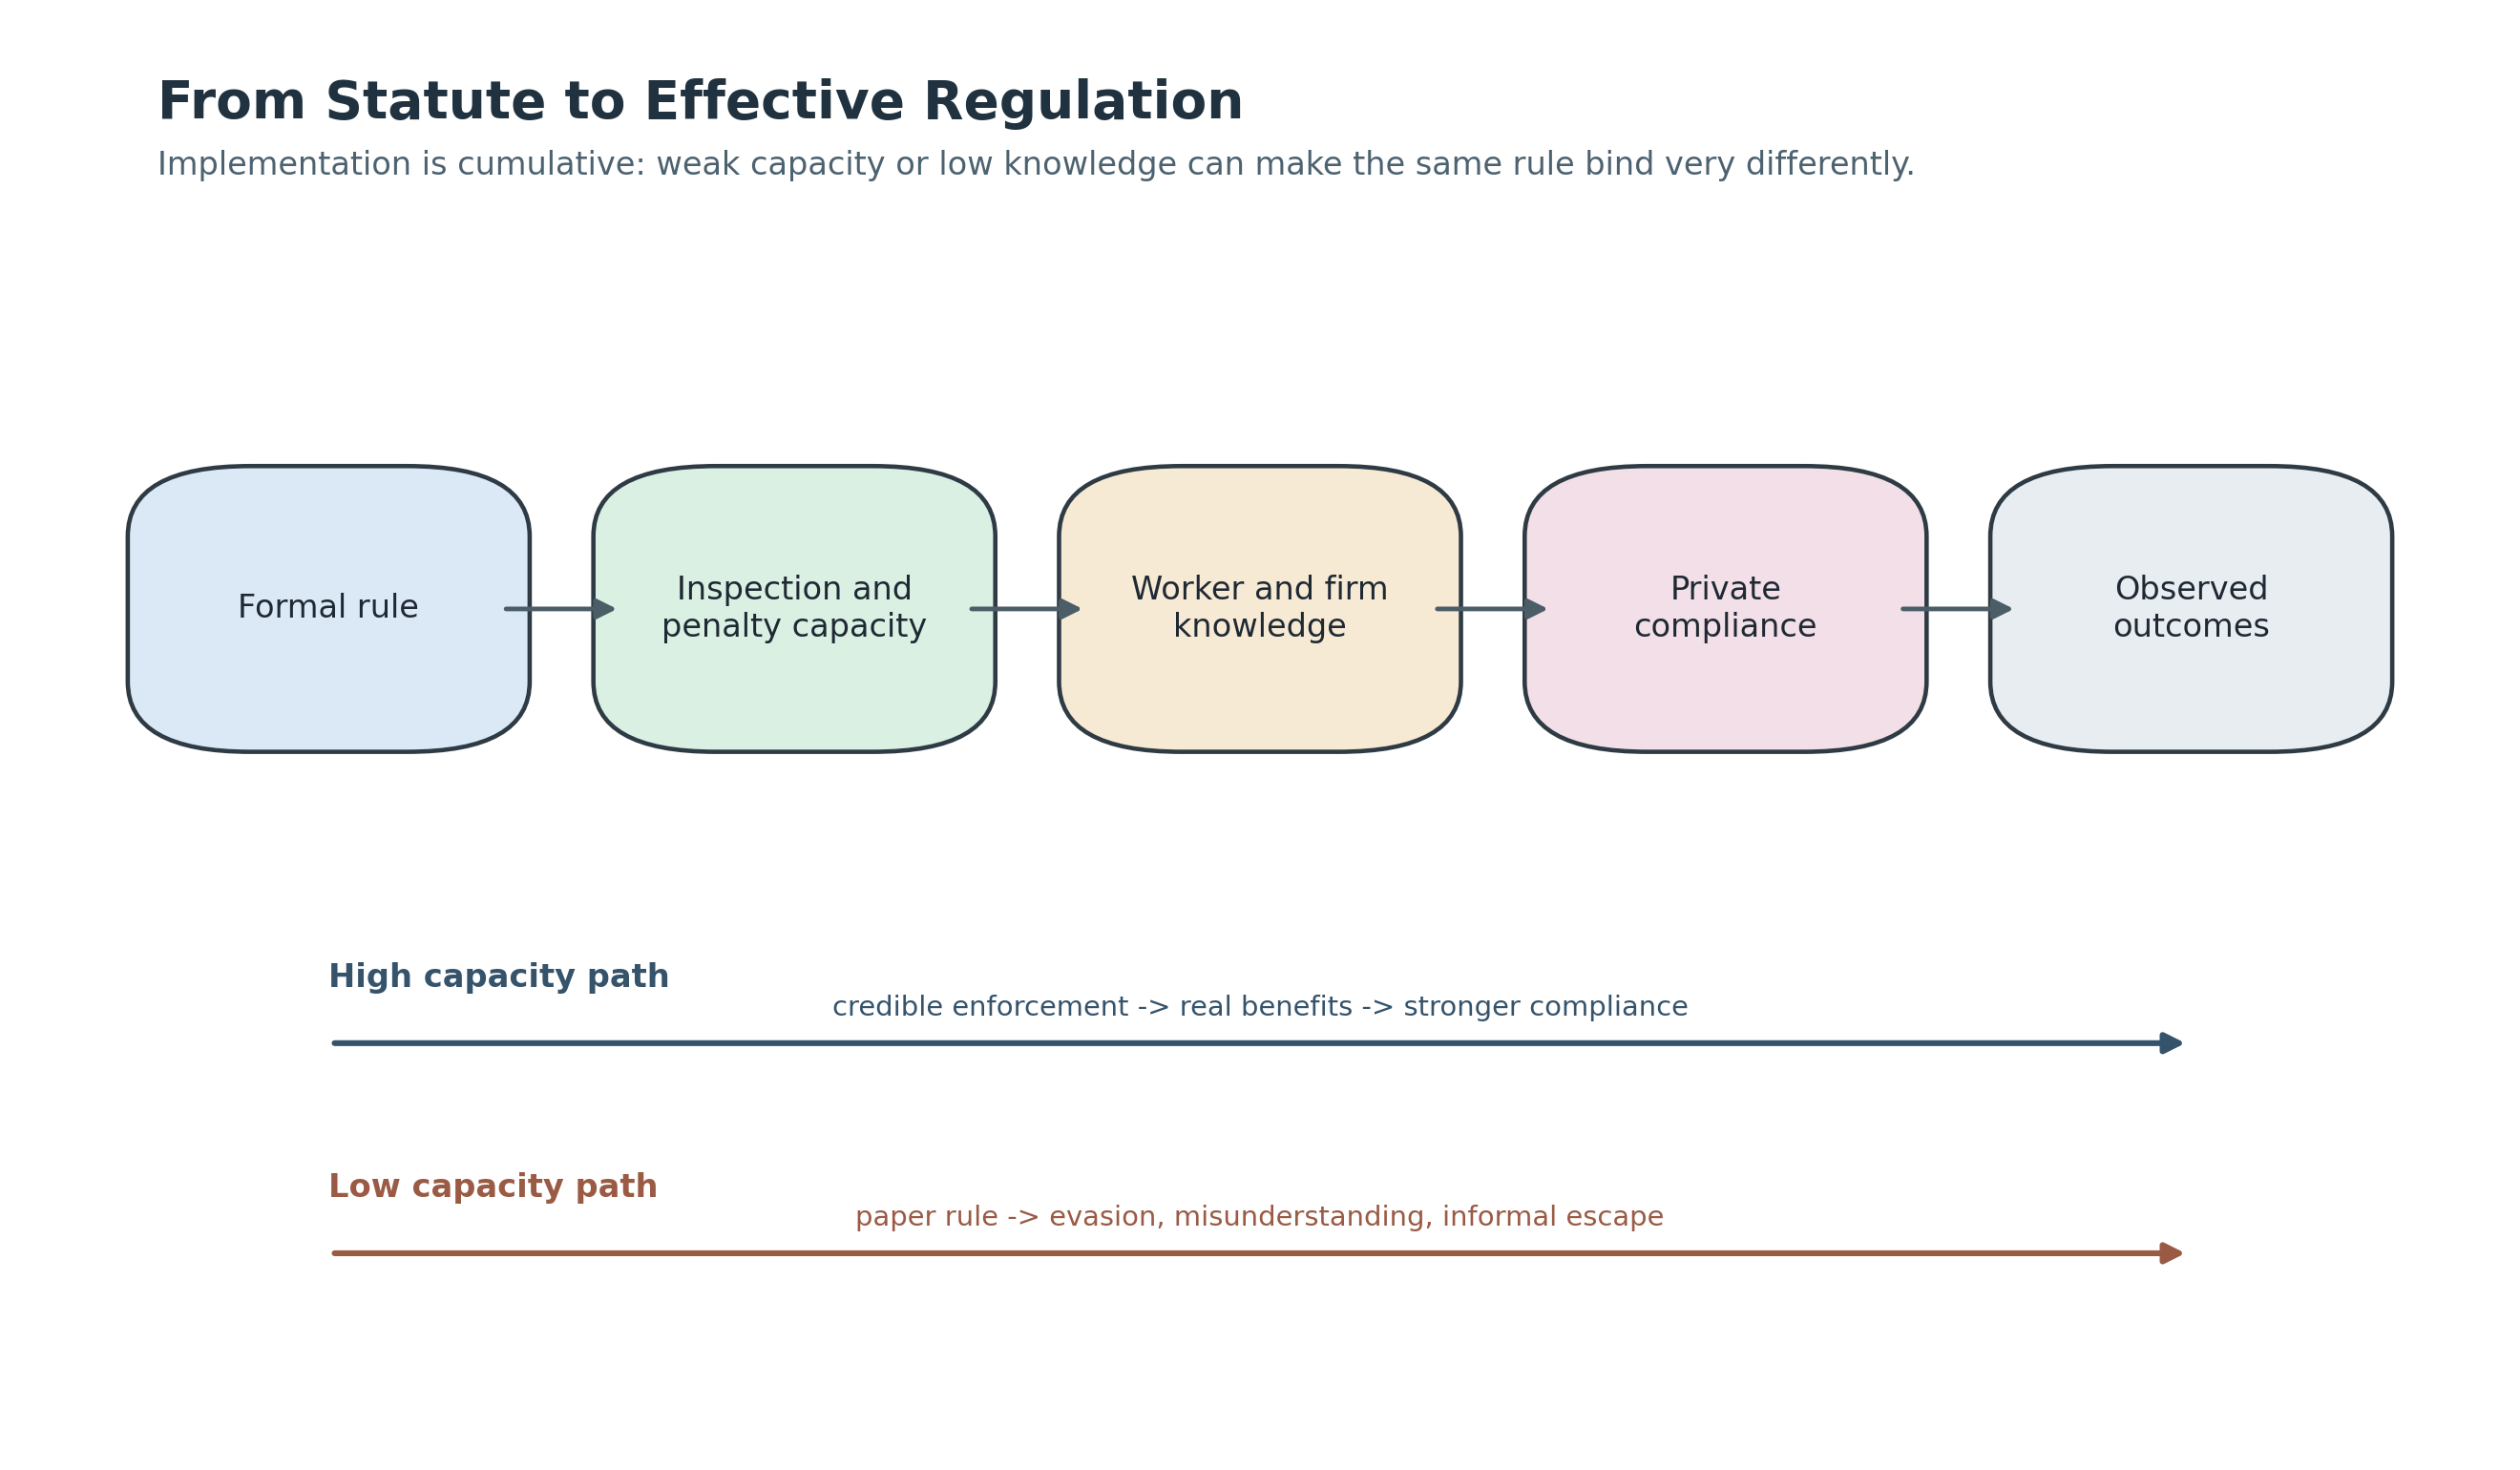
\includegraphics[height=0.74\textheight]{09-enforcement-capacity-to-effective-regulation.png}
\end{center}
\end{frame}

\begin{frame}{Insurance and equilibrium effects}
\[
\Delta W = MI - BD + EE
\]

\begin{itemize}
    \item $MI$: mechanical insurance gain.
    \item $BD$: behavioral distortion cost.
    \item $EE$: equilibrium externality on vacancies, nonrecipients, queueing, or informal work.
    \item UI is not only a recipient policy once labor-market tightness moves.
\end{itemize}
\end{frame}

\begin{frame}{Insurance, distortions, and uncovered margins}
\begin{center}
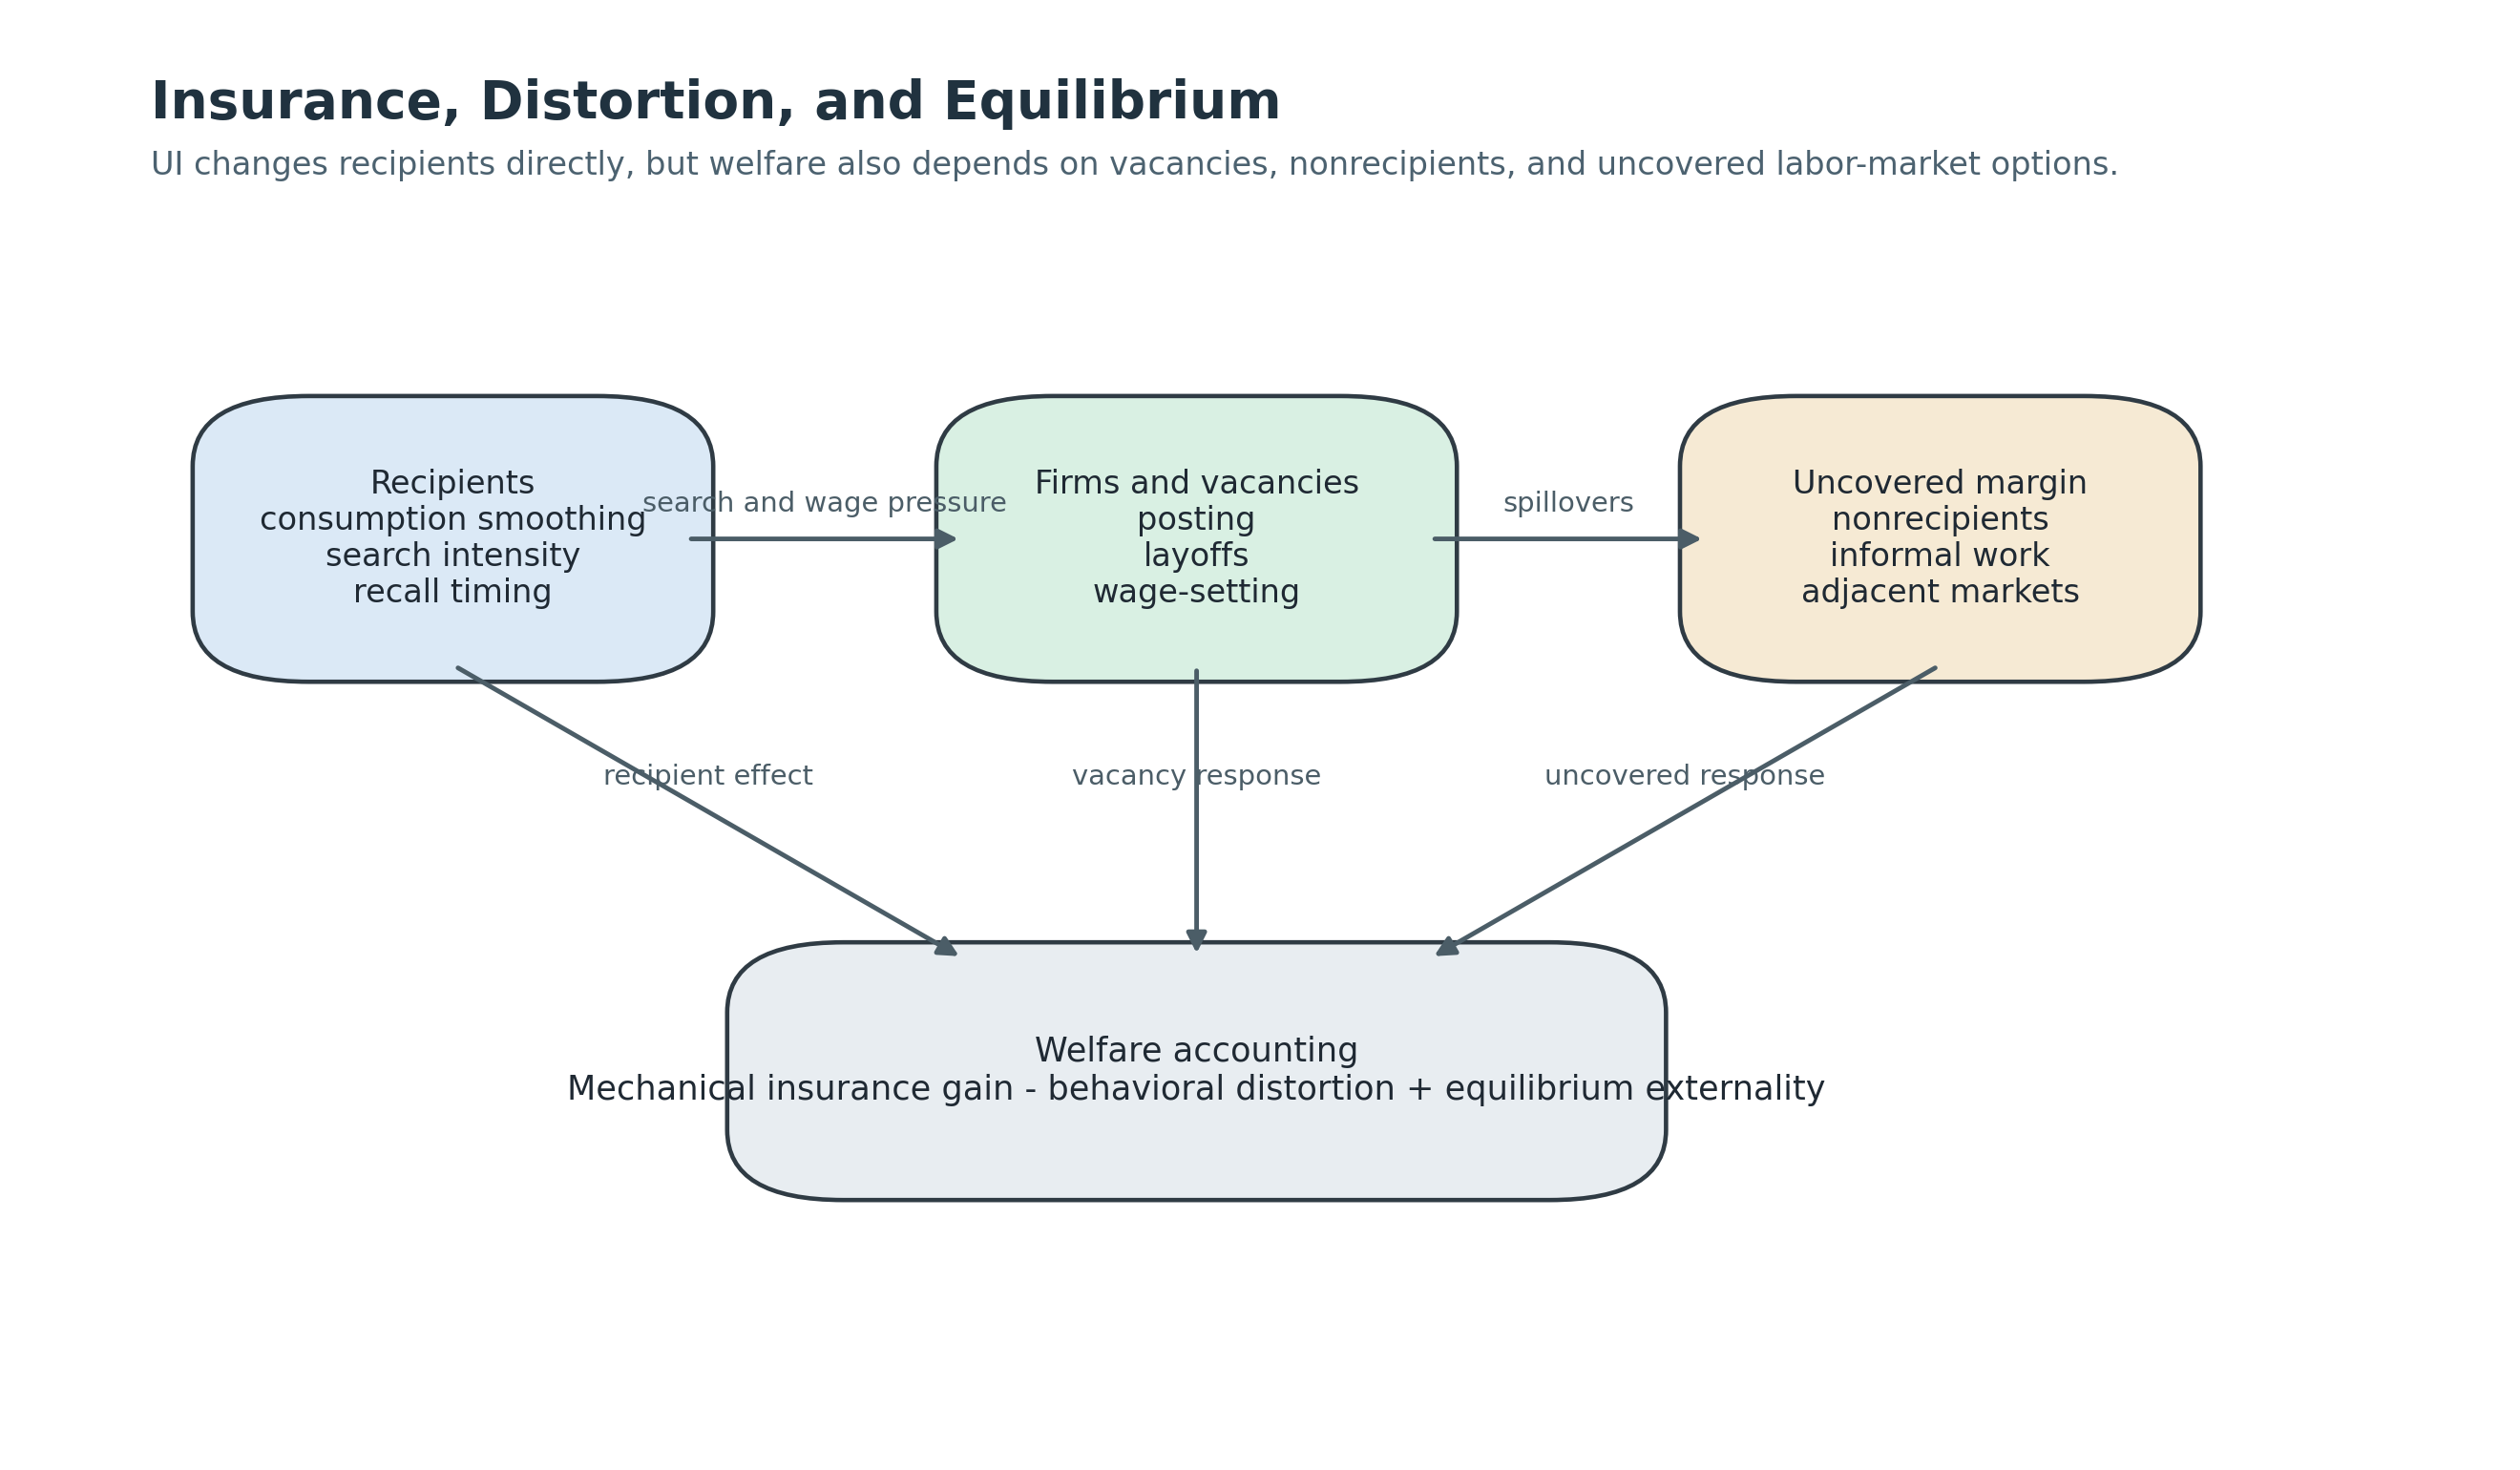
\includegraphics[height=0.74\textheight]{09-insurance-distortion-equilibrium.png}
\end{center}
\end{frame}

\begin{frame}{Information, transparency, and rights salience}
\begin{itemize}
    \item Information can change behavior even when formal legal rights do not change.
    \item Bertrand-Cr\'epon: labor-law advice shifts firm beliefs and employment.
    \item Cullen: pay transparency can change bargaining, coworker gaps, search, and employer competition.
    \item Information-based regulation belongs inside labor economics because it changes outside options, complaints, and wage-setting.
\end{itemize}
\end{frame}

\begin{frame}{Empirical designs and what they identify}
\small
\begin{tabular}{p{0.19\linewidth} p{0.18\linewidth} p{0.22\linewidth} p{0.28\linewidth}}
\toprule
Design & Unit & Best object & Main latent channel \\
\midrule
Legal reform / event study & State-year / worker-region & doctrine or statutory change & bundled reforms and trends \\
Threshold / kink & Worker spell & local insurance or eligibility effect & behavior away from cutoff \\
Enforcement shock & Firm / locality & effective regulation & endogenous state capacity \\
Information intervention & Firm / worker & beliefs, salience, complaints & diffusion and redesign \\
Equilibrium design & Region / market & spillovers on untreated workers & full market counterfactual \\
Formal-informal transition & Worker spell / locality & uncovered-margin adjustment & value of informal options \\
\bottomrule
\end{tabular}
\end{frame}

\begin{frame}{Effectiveness, spillovers, inequality, and welfare}
\begin{center}
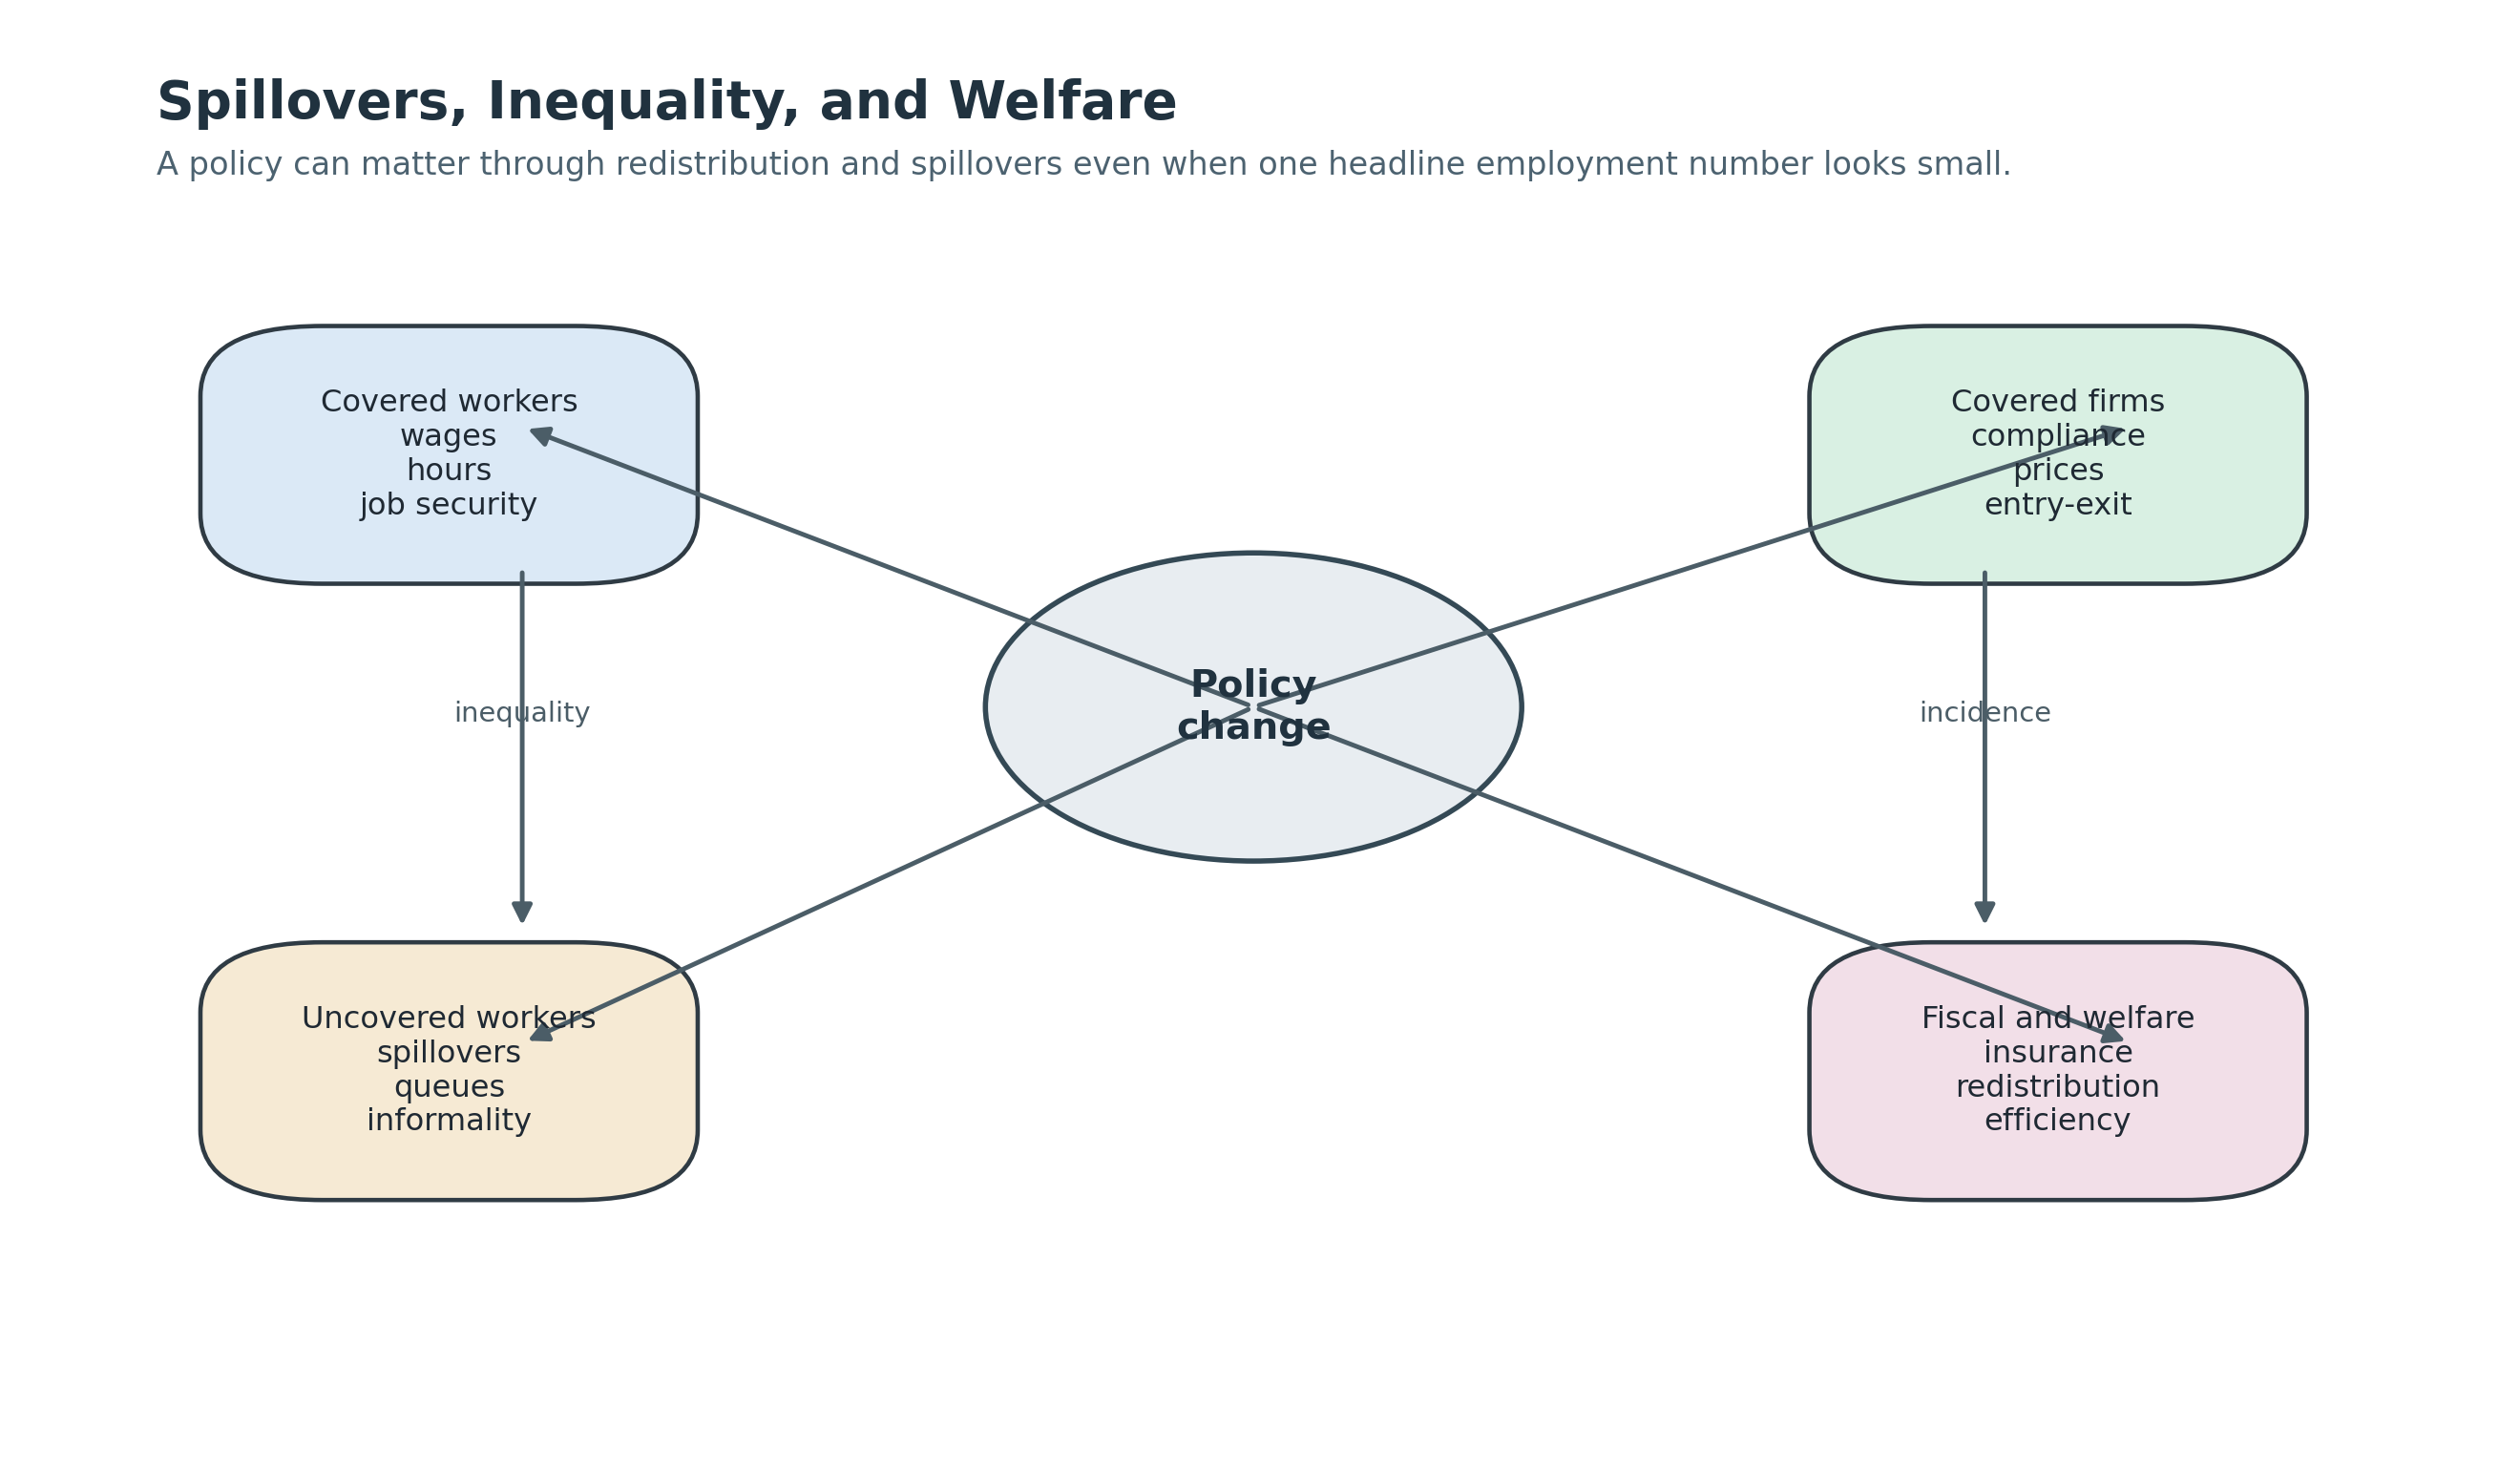
\includegraphics[height=0.66\textheight]{09-regulation-spillovers-inequality-welfare.png}
\end{center}
\begin{itemize}
    \item Small employment effects do not imply small welfare effects.
    \item Distribution, insurance value, price incidence, and uncovered workers matter.
\end{itemize}
\end{frame}

\begin{frame}{Why papers disagree}
\begin{itemize}
    \item They study different regulations.
    \item Enforcement regimes differ.
    \item Uncovered margins differ.
    \item Equilibrium assumptions differ.
    \item Welfare criteria differ.
\end{itemize}
\end{frame}

\begin{frame}{Bridge to Week 10 aggregate adjustment}
\begin{itemize}
    \item Dismissal rules shape layoffs, recalls, and hiring.
    \item UI changes vacancy posting, queueing, and unemployment duration.
    \item Enforcement capacity shapes formal versus informal adjustment.
    \item Information changes search and wage competition.
    \item Week 10 scales these institutional mechanisms up to aggregate shocks.
\end{itemize}
\end{frame}

\begin{frame}{Takeaways}
\begin{itemize}
    \item Labor regulation is best studied as a framework linking wedges, implementation, and equilibrium adjustment.
    \item Law on the books is never enough; enforcement, knowledge, and compliance are part of the treatment.
    \item Covered and uncovered margins must be analyzed together.
    \item Welfare depends on insurance, distortion, redistribution, and market structure, not only on employment.
\end{itemize}
\end{frame}

\appendix

\begin{frame}{Appendix: Week 9 lab bridge}
\begin{itemize}
    \item Reproduce: an Almeida-Carneiro style enforcement and formality panel.
    \item Diagnose: why a partial-equilibrium enforcement estimate differs from a Lalive-Landais-Zweimueller equilibrium UI estimate.
    \item Transfer: synthetic UI spillover and formality-margin designs.
    \item Keep the object explicit: dismissal, standards, enforcement, insurance, or information.
\end{itemize}
\end{frame}

\end{document}
